\documentclass[usenames,dvipsnames,aspectratio=169,table]{beamer}
%\usetheme{cern}
\usetheme{cernomc}

\usepackage{scrextend}
\changefontsizes{8pt}

% Beamer Setup ---
\setbeamercovered{transparent=5} 
\setbeamertemplate{navigation symbols}{} 

\AtBeginSection{%
	\begin{frame}[noframenumbering]{Outline}
	\tableofcontents[currentsection]
	\end{frame}
}

% Imports ---
\usepackage[utf8]{inputenc}
\usepackage{amsmath}
\usepackage{amsfonts}
\usepackage{amssymb}
\usepackage{unicode-math}
\usepackage{mathtools}
\usepackage{bm}  % bold math
\usepackage{graphicx}
\usepackage{grffile}  % filenames with dots 
\usepackage{fontawesome5}
\usepackage{minted}

\usepackage{tikz}
\usetikzlibrary{calc}

\usepackage{hyperref}
\usepackage{siunitx}
\usepackage{booktabs}
\usepackage{multirow}
\usepackage{caption}
\usepackage[absolute,overlay]{textpos}

\usepackage{fontspec}
\usefonttheme{serif}
%\setmainfont{STIX Two Text}
%\setmathfont{STIX Two Math}
\setmainfont{TeX Gyre Bonum}
\setmathfont{TeX Gyre Bonum Math}
\setmonofont{Fira Code}


% some shenanigans -------------------------------------------------------------
\newcommand{\highl}[1]{\textbf{#1}}
\definecolor{RunTwored}{RGB}{200,0,0}
\definecolor{APJgreen}{RGB}{20,150,0}
\definecolor{SbSorange}{RGB}{240,150,0}
\newcommand{\we}{\cellcolor{blue!20!white}}
\newcommand{\ho}{\cellcolor{red!20!white}}
\newcommand{\wh}{\cellcolor{green!20!white}}
\newcommand{\bonelabel}{%
        \node at ($(b1) +(-0.13\linewidth, 0.15\linewidth)$) {\sffamily\small\textbf{Beam 1}};
}
\newcommand{\btwolabel}{%
        \node at ($(b2) +(-0.13\linewidth, 0.15\linewidth)$) {\sffamily\small\textbf{Beam 2}};
}

\renewcommand{\theFancyVerbLine}{\textcolor[rgb]{0.5,0.5,1.0}{\scriptsize\arabic{FancyVerbLine}}}


% Meta -------------------------------------------------------------------------
\author[awegsche]{Andreas Wegscheider\\[1em]%
%
%\centering%
%
\includegraphics[width=3cm]{OMC_logo_original.pdf}%
}
\title[Magnet sorting]{Magnet sorting strategy}
\logo{} 
\titlegraphic{%

\includegraphics[width=3cm]{OMC_logo_original.pdf}%
    }
\institute{CERN}
\date[18.10.23]{18.10.2023}
\subject{} 

% Document ---------------------------------------------------------------------
\begin{document}

\begin{frame}
    \titlepage
\end{frame}

% --------------------------------------------------------------------------------------------------

\begin{frame}
    {Magnet sorting and pairing, cf EDMS 2912331}

    \begin{itemize}
        \item Field errors in superconducting magnets unavoidable
        \item Mitigation strategies to improve initial conditions: pairing and sorting of triplet quads
        \item Cryogenic requirements and tunnel layout impose limitations on possible sorting/pairing configurations
    \end{itemize}

    \textbf{Sorting}
    
    Triplet magnets (Q1, Q3) can be swapped between IP (1 <-> 5), side(L <-> R) and position within triplet (Q1 <-> Q3).

    \textbf{Pairing}

    Triplet magnets consist of two cold masses (A and B). For Q2, those can be swapped. 

    \textbf{Assembly Phases}

    Assembly takes place in three phases, configuration possibilities decrease in each phase.

\end{frame}
% --------------------------------------------------------------------------------------------------

\begin{frame}
    {Assembly Phases}

    From \texttt{EDMS 2912331}:\\[0.5em]

    \begin{tabular}{c|l|r}
        \textbf{Phase} & \textbf{Description} & \textbf{Number of possibilities}\\
        \hline
        1 & 8 possibilities for Q1/Q3 & $8! = 40320$\\
          & 8 possibilities for Q2a/b & $8! = 40320$\\
          \hline 
          & sum                       & $80640$\\
          \hline 
          \hline 
        2 & 8 possibilities for Q1/Q3 & $8! = 40320$\\
          & 4 possibilities for Q2a   & $4! = 24$\\
          & 4 possibilities for Q2b   & $4! = 24$\\
          \hline 
          & sum                       & $40368$\\
          \hline 
          \hline 
        3 & 2 possibilities for Q1   & $2! = 2$\\
          & 2 possibilities for Q3   & $2! = 2$\\
          & 2 possibilities for Q2   & $2! = 2$\\
          \hline 
          & sum                       & $6$\\
          \hline 
          \hline 
    \end{tabular}
\end{frame}

% --------------------------------------------------------------------------------------------------

\begin{frame}[fragile]
    {Current status}


    \begin{minipage}{0.45\linewidth}
    \begin{itemize}
        \item Setup simulation scripts to \highl{introduce errors} and \highl{control sorting}\\
        \item Ran extensive simulations with \highl{naive} sorting methods
        \item Recorded correctability using omc3's \texttt{global\_correct}
        \item All code available at \\ 
            {\small \faGithub~\href{https://github.com/awegsche/magnet_sorting}{\texttt{magnet\_sorting}}}
    \end{itemize}
    \end{minipage}
    \hfill
    \begin{minipage}{0.52\linewidth}
        Example usage:
        \small
        \begin{minted}
            [
            numbersep=5pt,
            fontsize=\footnotesize,
            linenos,
            bgcolor=blue!5!white,
            ]
            {python}
q2_errors = Q2Pairs(real_errors=10,
                    meas_errors=2,
                    stage=1)

# apply sorting on sum
q2_errors.sort_sum()

# write errors to madx file
q2_errors.write_errors_to_file("errors_Q2.madx")

# run madx, run global_correct, compare outputs
# ...
        \end{minted}
    \end{minipage}
\normalsize
    
\end{frame}

% --------------------------------------------------------------------------------------------------

\begin{frame}[fragile]
    {Simulation steps}

    for each seed:

    \begin{itemize}
        \item Generate initial errors ($\delta K_1 / K_1 = 50\times 10^{-4}$)
        \item \texttt{twiss} of initial lattice
        \item Perform (simulated) analysis and correction of initial lattice
        %\item if $\beta$~beating is too low or lattice failed, disregard this seed, record as failed
        \item If "correctable", perform sorting according to selected method
        \item \texttt{twiss} of sorted lattice
        \item Perform (simulated) analysis and correction of sorted lattice
        \item Record $\beta$~beating
    \end{itemize}


    Sample record summary:\hspace{2em}
    \begin{minipage}[t]{0.6\linewidth}
    \footnotesize
    \begin{verbatim}
Simulation Summary
==================
not correctable :       0 (   0%)
low beta beat   :     100 (  20%)
general failed  :       0 (   0%)
passed          :     400 (  80%)
--------------------------------
total           :     500
    \end{verbatim}
    \normalsize
        \end{minipage}

    
\end{frame}

% --------------------------------------------------------------------------------------------------

\begin{frame} % ------------------------------------------------------------------------------------
    {Effect on correction quality}


    Plots show $\beta$~beating after correction, before and after sorting.

    Sorting method: sort on \texttt{sum}, assuming that errors of neighbouring quads can self-compensate.
    
    \begin{center}
        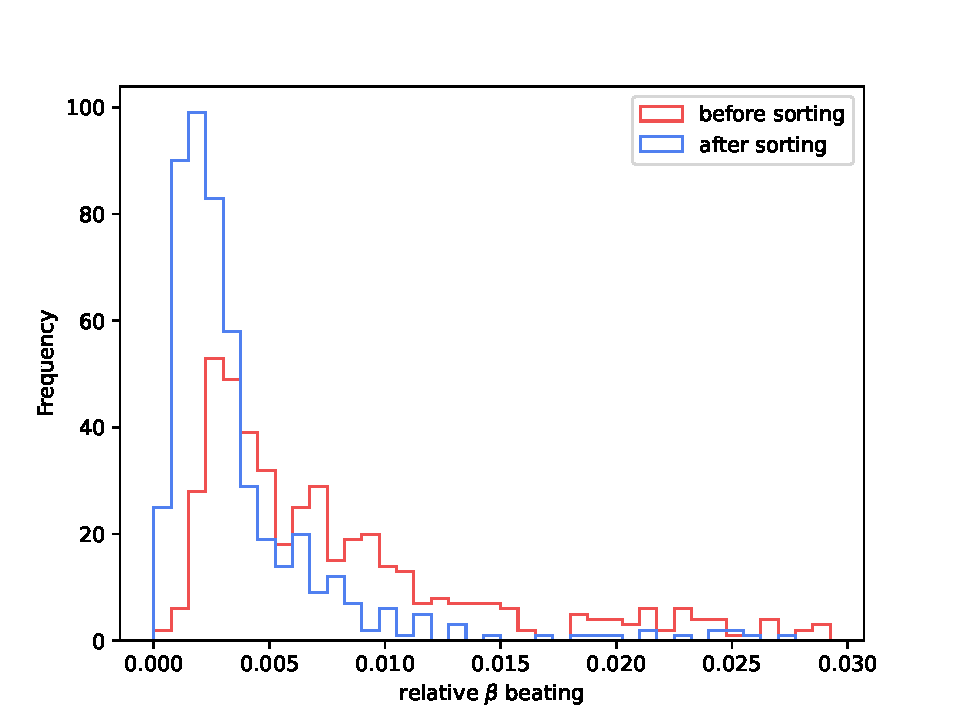
\includegraphics[width=0.5\linewidth]{recon_threshold.pdf}
    \end{center}

\end{frame} % --------------------------------------------------------------------------------------

\begin{frame} % ------------------------------------------------------------------------------------
    {Effect on correctability}

    

    \begin{center}
    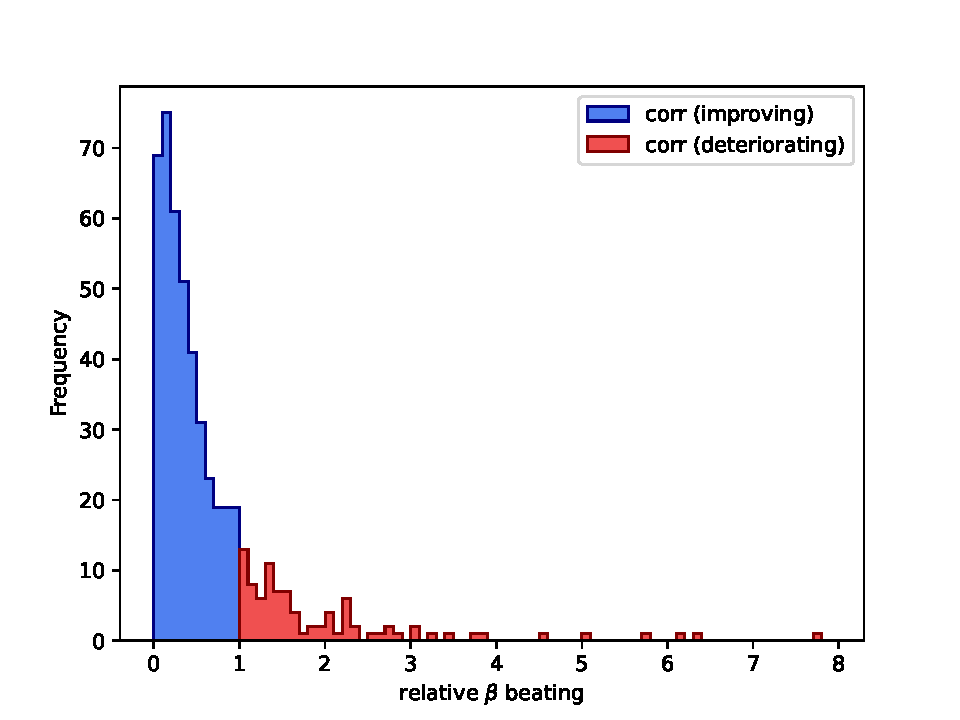
\includegraphics[width=0.6\linewidth]{corr_threshold.pdf}
    \end{center}

\end{frame} % --------------------------------------------------------------------------------------


\begin{frame} % ------------------------------------------------------------------------------------
    {Correlation}

    \begin{minipage}{0.6\linewidth}
        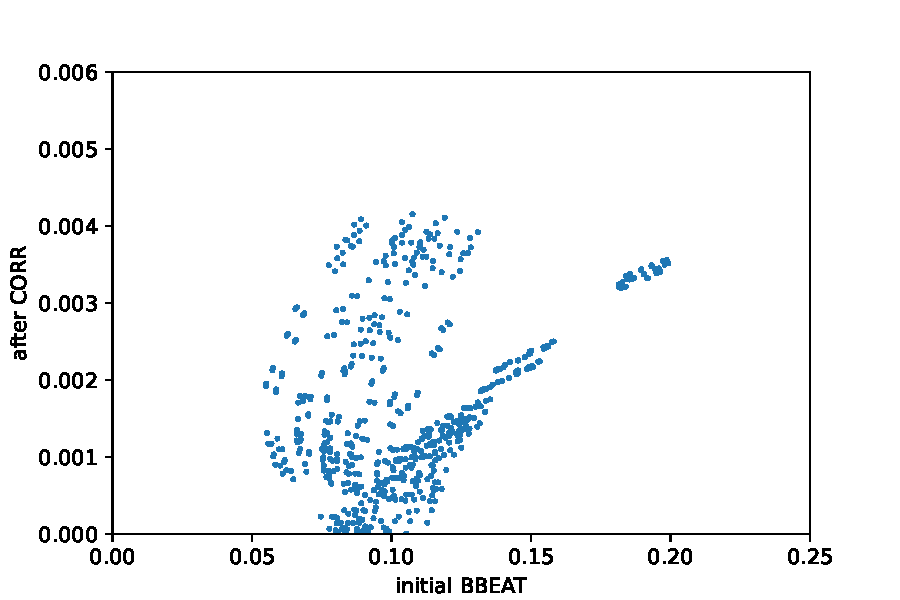
\includegraphics[width=\linewidth]{correlation_full.pdf} 
    \end{minipage}
    \begin{minipage}{0.39\linewidth}
        Some correlation but also filaments with no correlation.

        \textbf{To be investigated}

    \end{minipage}
    
\end{frame} % --------------------------------------------------------------------------------------


\begin{frame} % ------------------------------------------------------------------------------------
    {Current work / future plans}


    \begin{itemize}
        \item Get more statistics (all stages of assembly process, different sorting criteria)
        \item Introduce measurement uncertainty
    \end{itemize}
    
\end{frame} % --------------------------------------------------------------------------------------
% \backcover

\end{document}
